\documentclass[12p]{article}

\usepackage{geometry} % Requied to change the page size to A4
\geometry{a4paper} % Set the page size to be A4 as opposed to the default US Letter

\usepackage[utf8]{inputenc}
\usepackage{graphicx}
\usepackage{float} % Allows putting an [H] in \begin{figure} to specify the exact location of the figure
\usepackage{wrapfig} % Allows in-line images such as the example fish picture
\usepackage[nopar]{lipsum} % Used for inserting dummy 'Lorem ipsum' text into the template
\usepackage{fancyhdr}
\usepackage[parfill]{parskip} % Makes sure to put line breaks in between paragraphs and have no indentation
\usepackage{dirtytalk} % Used for quotations (\say{quote})
\usepackage[toc,page]{appendix}
\usepackage{caption}
\usepackage{subcaption}
\usepackage{url}
\usepackage{minted} % Used for including code with syntax highlighting: https://www.sharelatex.com/learn/Code_Highlighting_with_minted
\usepackage{fontawesome} % Allows usage of icons within text
\usepackage{enumitem}
\usepackage[final]{pdfpages}

\usepackage[
 style=numeric,
 sorting=none
 ]{biblatex}
\addbibresource{references.bib}

\linespread{1.2} % Line spacing
\setlength\parindent{0pt} % Globally suppress indentation
 
\graphicspath{{pics/}} % Specifies the directory where pictures are stored

\pagestyle{fancy} % Use this, if a header on each page with the section title and page number is wanted
\fancyhf{} % Removes all headers and footers, comment this to show page number at the bottom of each page again
\fancyhead[L]{\rightmark} % Sets the section title on the left side of the header
\fancyhead[R]{\thepage} % Sets the page number on the right side of the header

\newcommand{\HRule}{\rule{\linewidth}{0.5mm}} % Defines a new command for horizontal lines
\newcommand{\SlimHRule}{\rule{\linewidth}{0.25mm}} % Defines a new command for horizontal lines


%----------------------------------------------------------------------------------------

\begin{document}

%----------------------------------------------------------------------------------------
%	TITLE PAGE
%----------------------------------------------------------------------------------------

\begin{titlepage}
	 
	\center
	 
	%------------------------------------------------
	%	Logo
	%------------------------------------------------
		
	
\includegraphics[width=0.2\textwidth]{pics/AAU_Logo.png}\\[1cm]
		 
		%------------------------------------------------
		%	Headings
		%------------------------------------------------
			
		\textsc{\LARGE Aalborg University Copenhagen}\\[1.5cm]
			
		\textsc{\Large P2 Project}\\[0.5cm]
			
		\textsc{\large Group 4}\\[0.5cm]
			
		\textsc{\large IT, Communication and New Media}\\[0.5cm]
			
			
		%------------------------------------------------
		%	Title
		%------------------------------------------------
			
		\HRule\\[0.4cm]
			
		{\huge\bfseries Cartographer}\\[0.4cm]
		
		\HRule\\[0.4cm]
			
		%{\huge\bfseries This page will be replaced with AAU's sample header page}\\[0.4cm]
			
		%------------------------------------------------
		%	Author(s) and Supervisor(s)
		%------------------------------------------------
			
		\begin{minipage}{0.4\textwidth}
			\begin{flushleft} \large
				\emph{Authors}\\
				Ludvig Alexander \textsc{Brüchmann} \\
				Johannes \textsc{Mols} \\
				Agata \textsc{Surmacz} \\
				Ricardo \textsc{Yaben} \\
				Boris \textsc{Yordanov} \\
				Benas \textsc{Zauka} \\
			\end{flushleft}
		\end{minipage}
		~
		\begin{minipage}{0.4\textwidth}
			\begin{flushright} \large
				\emph{Study Numbers} \\
				20174692 \\
				20174921 \\
				2017xxxx \\
				2017xxxx \\
				2017xxxx \\
				20173806 \\
			\end{flushright}
		\end{minipage}\\[0.5cm]
		 
		%------------------------------------------------
		 
		\begin{minipage}{0.4\textwidth}
			\begin{flushleft} \large
				\emph{Supervisors}\\
				Jannick Kirk \textsc{Sørensen} \\
				Sokol \textsc{Kosta} \\
			\end{flushleft}
		\end{minipage}
		~
		\begin{minipage}{0.4\textwidth}
			\begin{flushright} \large
			\end{flushright}
		\end{minipage}\\[0.5cm]
		
		%------------------------------------------------
		%	Date
		%------------------------------------------------
			
		\vfill\vfill\vfill % Position the date 3/4 down the remaining page
			
		{\large\today} % Date, change the \today to a set date if you want to be precise
			
		\end{titlepage}
		
		%----------------------------------------------------------------------------------------
		%	SYNOPSIS / ABSTRACT
		%----------------------------------------------------------------------------------------
		
		\begin{abstract}
			\thispagestyle{plain} %Sets the page style for this specific page to plain, to remove the header and show the page number at the bottom
			
			\noindent This is our abstract
			\newline \newline
			\noindent ...
			
		\end{abstract}
		
		\newpage
		
		%----------------------------------------------------------------------------------------
		%	TABLE OF CONTENTS
		%----------------------------------------------------------------------------------------
		
		\tableofcontents % Include a table of contents
		\thispagestyle{plain} %Sets the page style for this specific page to plain, to remove the header and show the page number at the bottom
		
		\newpage % Begins the report on a new page instead of on the same page as the table of contents 
		
		%----------------------------------------------------------------------------------------
		%	INTRODUCTION
		%----------------------------------------------------------------------------------------
		
		\section{Introduction}
		
		\subsection{Problem introduction} \label{ProblemIntroduction}
		
		This project specifically focuses on Google and their Google Maps service. With Android having a market share of 75\% in 2017, according to IDC \cite{SmartphoneOSMarketShare}, and Google Maps being pre-installed on every Android device, Google can collect location-based information on a big portion of humanity. In fact, more than 2 billion persons \cite{AndroidMonthlyActiveUsers}, as Google announced in 2017.
		
		As an attempt to give users access to their own data, Google launched "Latitude" in 2009 \cite{GoogleLatitude}. This was a web and mobile app, that tracked your location and shared it with your contacts. This project was retired in 2013. Snapchat, yet another major social media player, released a similar feature on their platform in 2017 \cite{SnapchatMap}. Both of those projects raised a lot of concern about user privacy.
		
		In 2015, Google announced a comeback of the location history \cite{TimelineAnnouncement}. However, this feature keeps the user's data private and only visible to the user itself. This timeline tracks a users movement at all times, and can even determine which kind of transportation he or she used. The user can then view their timeline for each day.
		
		Unfortunately, the timeline only shows a single day at once and doesn't deliver in-depth statistics or other useful information. And this is where this project kicks in. 
		
		Google lets users download their raw location history as a file, containing bare coordinates, timestamps and presumed activities (like riding a bike, taking the train, etc.). The application behind this project focuses on extracting this data and giving the user an overview of what is being tracked and what the data says about them.
		
		\subsection{Problem formulation} \label{ProblemFormulation}
		
		What information can you extract from the data that Google is collecting from you, specifically the location history? How can we use that data for the user’s benefit? Would users be interested in getting useful advice collected from that data?
		
		
		\subsection{Project delimitations} \label{ProjectDelimitations}
		
		This report will not go into market or business analysis of any kind since this project is supposed to be a free and open-source tool to analyse user data. We are not considering to start a business based on this, nor to monetise the app in any way.
		
		Furthermore, privacy won't be part of this report either, as this is a big problem and will be addressed in the fifth semester of ITCOM. However, we will still address privacy matters regarding the data that is being collected by Google, since this is the foundation of this project.
		
		\subsection{Project introduction} \label{ProjectIntroduction}
		
		Due to increasing advantages brought upon by active developments in various technology, the world has gained a new level of mobility. This was made possible by the steady process of globalisation. As such, technology plays a key role in today's society. Using such technology, both the developers and the users are able to collect, maintain and access sensitive information and data, stored about the user within personal technology, which includes information such as whereabouts (visited locations, areas of visit within a specific time of day/date, etc.), interests, etc. An existing practice of abusing such information is especially predominant online, and used in unison with ads.
		
		Google collects your personal data in order to target ads, as well as to improve your experience when using a specific device. Here are some of the things Google most likely knows about you, if you use your device frequently:
		\begin{itemize}
			\item Your name, gender and birth date
			\item Your personal cellphone number(-s)
			\item Your contacts list
			\item Your recent Google searches
			\item Websites that you have visited
			\item Where you have been, since you have a phone with Google Maps
			\item Your interests
			\item Where you work and your home address
		\end{itemize}
		
		And these are just a couple of things, there are many more to name
		
		\textbf{add fluff}
		
		\textbf{insert pic of Google’s Location History page}
		
		However, the way to access this information is not equally as easy for the developers and the users. As such, the goal of our project is to create an application that grants you access to the information Google receives and stores for you, and use it for personal benefit. To be more precise, we want to take information that Google stores about your past and present locations and make it easily accessible via heat maps, graphs and diagrams: we want to take Google's Location History page and make it more comfortable to use, as well as to bring attention to the fact that the access to such information is not limited to just the developers.
		
		
		%----------------------------------------------------------------------------------------
		%	METHODOLOGY
		%----------------------------------------------------------------------------------------
		
		\newpage
		\section{Methodology} \label{Methodology}
		
		    \subsection{Brainstorming}
		
    		\subsection{Project management}
    		
    		\subsection{State of the Art}
    		Explain how we learned about Google's tracking, existing solutions
    		
    		\subsection{Location History}
    		Explain the JSON's structure and content
    		
    		\subsection{Database}
    		Explain choice of db and encryption
    		
    		\subsection{Application Design}
    		Project visualisation is very important in that it creates the foundation for the entire process flow. Without a sketch, or a draft, working on a single application in a group of individuals would be almost impossible, as everyone has different ideas of how a good application has to look and function. The right visualisation is crucial for follow-up decisions, the application’s structure and data analysis. For that reason, to ensure that all of us had mutual intentions and goals when it comes to the structure of this application, we decided to create desirable mock-up visuals for our application using the online services of the “Marvelapp” sketching app. In addition, as we wanted the application to be accessible to a broader scale of users, not just ones exclusively limited to mobile phones, despite them being the major demographic, we decided to develop the visualisation with tablet users in mind as well.
    		
    		\subsection{Implementation}
    		Finding the right APIs
    		Authentication
    		
    		\subsection{User Research}
    		It is highly important to make sure that an idea for an application is actually in demand by enough possible users. User research gives an insight into this demand, and can also bring important feedback on certain features, the application design, availability, price and more.
            
            In this case, we constructed an online survey/questionnaire \cite{Survey} with the Google Forms \cite{GoogleForms} service. The goal of this survey is to test participants on their awareness of location-related data collection, in particular by Google. The survey asks questions like \textit{"Do you believe your phone tracks your location?"} and follows up with questions about whether participants think that data is accessible to them and if they have ever seen it.
            
            The second part of the survey focuses on the participant's willingness to use our application, by asking them how comfortable they are with sharing their location history with our this third-party service, and what features they would like to see. The participants also get an option to not use our application, which is followed up by asking them what the reason for that is (e.g. privacy concerns, lack of interest, ...).
            
            For surveys to be meaningful, it is not only important to get many answers, but also to get diverse answers from different persons with different backgrounds. For this to work, the survey has to be shared on different platforms.
            
            The first and easiest way to distribute the survey is to post it on Facebook, in an AAU group made for this specific purpose. Furthermore, we distributed the survey on various different platforms (e.g. Surveycircle \cite{Surveycircle} and Poll Pool \cite{PollPool}).
    		
    		\subsection{Development Methodology}
    		
    		\subsection{Storyboarding}
    		Storyboarding is quite an important tool used in software development, used to identify specifications for a software. It is applied as visualisation of different scenarios that illustrate the important steps of the user experience. Said storyboard is then modified, based on specific individual needs of both the user and the manufacturer. The method of storyboarding is important because it is fast and cheap to produce, and it helps to finalise abstract ideas. In addition, said method is also beneficial to the user, providing a clear, visual depiction of how the software is supposed to function, and going to work.
    		
    		\subsubsection{Storyboard} <!--Gonna put it here for now -->
    		
    		The storyboard follows these six steps:
    		\begin{itemize}
    		    \item Attention
    		    \item Interest
    		    \item Desire
    		    \item Action
    		    \item Onboarding
    		    \item Retention
    		\end{itemize}
    		
    		<!-- describe the portrayed storyboard -->
    		
		%----------------------------------------------------------------------------------------
		%	STATE OF THE ART
		%----------------------------------------------------------------------------------------
    		
		\newpage
		\section{State of the Art} \label{sec:StateOfTheArt}
    		\subsection{Introduction}
		
		To further progress the development of the application, understanding Google and its ways of collecting and processing information is essential. As such, first and foremost, we’re going to look at Google’s policies regarding tracking user information.
        
        Google collects information in these ways: \cite{GooglePrivacyPolicy}
        
        1st: Pieces of information the userbase provides them through individual services. This is done through a sign-up process, where Google receives your personal information that includes your name, email, tel. number, credit card, etc.
        
        2nd: Collecting information through the use of services. This includes device-specific information (such as operating system, hardware model, etc.), log information (search queries, tel. log info., tec.), local storage, as well as location information (personal location, IP address, GPS, etc.), among other things.
        
        The central focus for us is the collection of information that is based on personal location. As mentioned beforehand, this can be done through things such as the IP address, GPS, as well as Wi-Fi access points and even cell towers. The accessibility of such information is quite tricky on the user’s end, however, as Google is not sufficiently transparent regarding displaying such information without the user having to go out of their way to self-research its access. Additionally, there are people who use such Google's services without the realisation that they’re sharing said information with the provider.
		
		Alas, we were able to identify several exemplary applications that allow the user base to access the location-based information that Google has stored on individual users.
		
		\newpage
    		\subsection{Competitiors}
    		\begin{itemize}
    			\item https://www.google.com/maps/timeline
    			\item https://locationhistoryvisualizer.com
    			\item http://theyhaveyour.info/
    		\end{itemize}
    		%------------------------------------------------
		
		\newpage
		\subsection{Conclusion}
		
		%----------------------------------------------------------------------------------------
		%	SYSTEM REQUIREMENTS
		%----------------------------------------------------------------------------------------
		
		\newpage
		\section{Requirements} \label{sec:Requirements}
		
		\subsection{User requirements} \label{sec:UserRequirements}
		
		\subsection{System requirements} \label{sec:SystemRequirements}
		
		%----------------------------------------------------------------------------------------
		%	ARCHITECTURAL DESIGN
		%----------------------------------------------------------------------------------------
				
	    \newpage
		\section{ArchitecturalDesign} \label{sec:ArchitecturalDesign}
		    \subsection{Context Diagram}
		    \subsection{Class Diagram}
		    \subsection{Sequence Diagram}
		    \subsection{Architectural Diagram}
		    \subsection{Use case Diagram}
		%----------------------------------------------------------------------------------------
		%	SOFTWARE DESIGN
		%----------------------------------------------------------------------------------------
		
		\newpage
		\section{Software design} \label{sec:SoftwareDesign}
		    \subsection{Introduction}
		    The sketches for the application were made using the online tool \textit{Marvelapp} \cite{Marvelapp}. We chose it because it has a varied library of pre-designed components which we were able to leverage to save time. It also allows sharing the sketches, multiple people to work on them and to export them.
		    For the actual components in the app we used the built-in Android library.
		    
    		\subsection{Introduction slides}
            \begin{figure}[ht]
                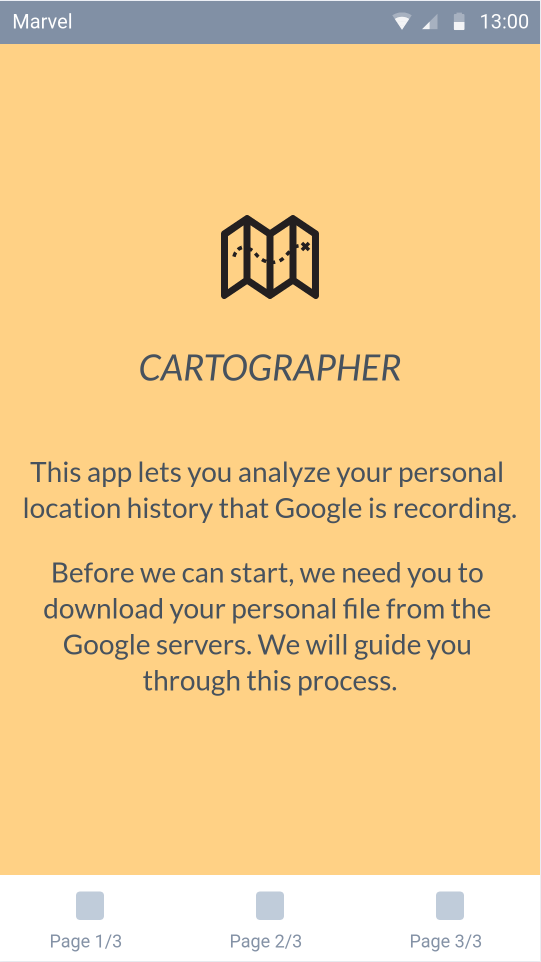
\includegraphics[height=8cm,keepaspectratio]{pics/app_design/intro.PNG}
        		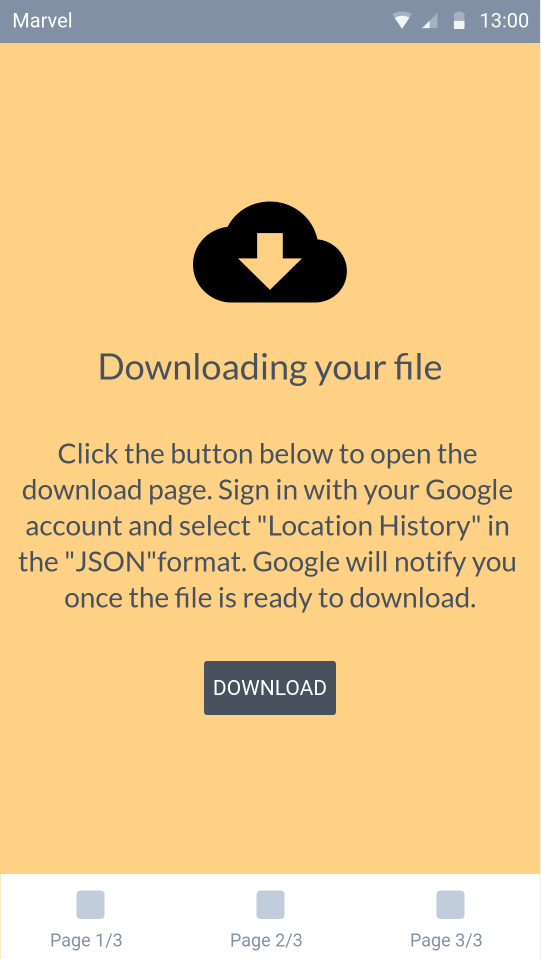
\includegraphics[height=8cm,keepaspectratio]{pics/app_design/intro2.PNG}
        		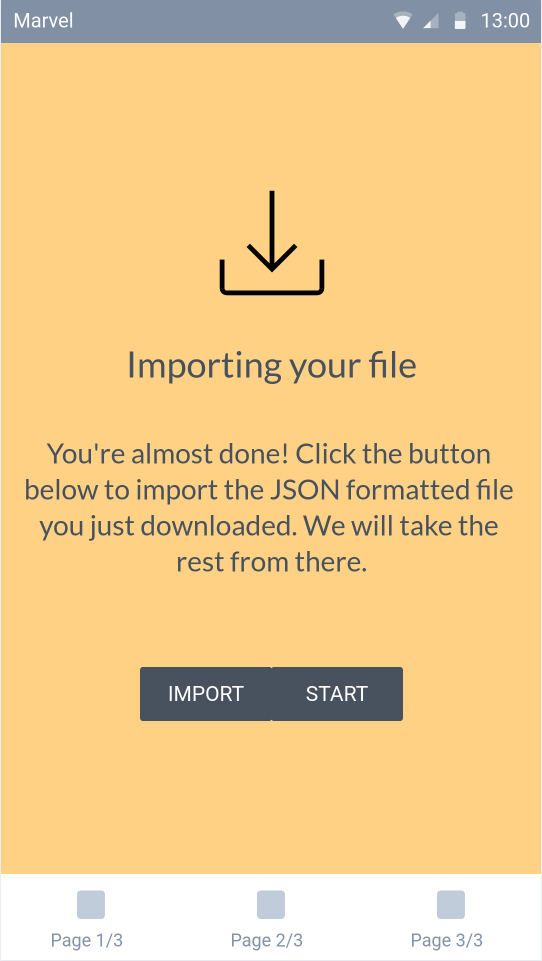
\includegraphics[height=8cm,keepaspectratio]{pics/app_design/intro3.PNG}
    		    \caption{Sketch of the introduction screens}
            \end{figure}
            
            The introduction slides are only shown once, at the first start of the application. The introduction consists of several slides that show various information about the application, what it does and what it needs.
            
            The first slide informs the user of the purpose of the application and what the user is required to do. After that, three slides with more text and a button each, appears. The first slide gives the user the possibility to visit the Google web page where he or she can download the personal location history file. When downloading, Google gives users a \texttt{.zip} file, which needs to be unzipped. This is the purpose of the next slide. Here, the user can select the downloaded archive and the application will automatically unzip it. On the final slide, the user is finally asked to import the \texttt{.json} file that was contained in the archive. While processing the file, a loading screen is shown.
    		
    		\subsection{Main dashboard}
    		\begin{figure}[ht]
    		    \center
                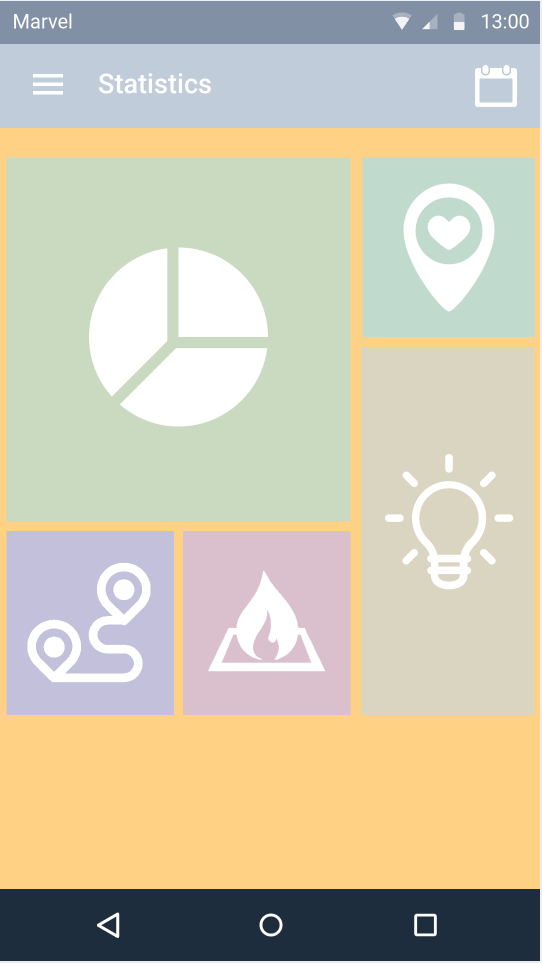
\includegraphics[height=8cm,keepaspectratio]{pics/app_design/main.PNG}
                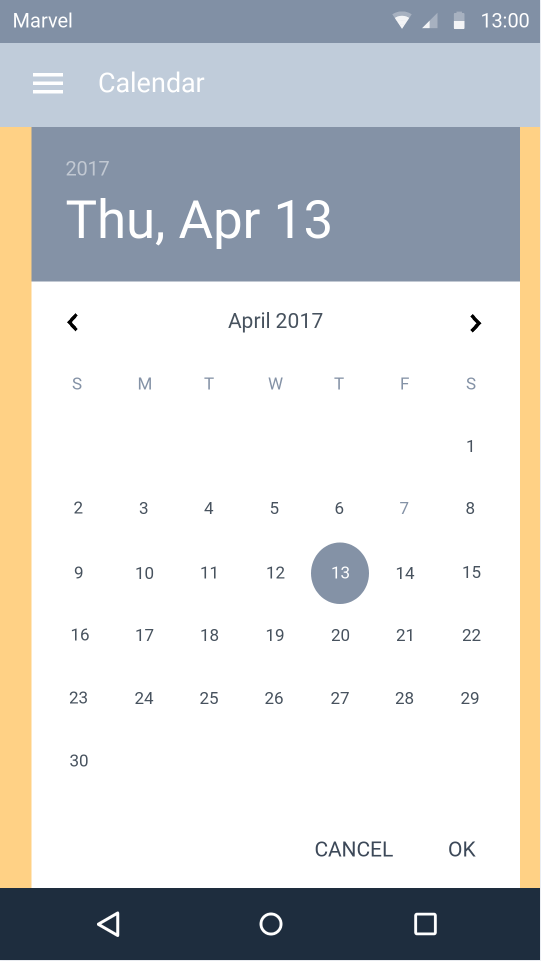
\includegraphics[height=8cm,keepaspectratio]{pics/app_design/calendar.PNG}
                \caption{Sketch of the main dashboard and calendar}
            \end{figure}
    		When the user uploads his or her \texttt{.json} file and the app opens, he is directed towards a screen full of diagrams, graphs and heatmaps. By pressing each one individually, he is able to access his information in a myriad of different selections: He can see how much time he has spent in different locations, he can access information on the routes he frequently travel on, how much time he spent going to said routes, how long he stays in certain locations and what transport he takes to get there, as well as the average distance he has travelled in total. In addition, he can select the calendar to change the duration of time the diagrams, graphs and heatmaps take his information into account (Example: If he selects a week, the application will display his records within that week).
    		
    		\subsection{Favourite routes}
    		In this section users can see routes they usually take. The routes are displayed as lines on a map, which are snapped to the roads.
    		
    		\subsection{Favourite places}
            
    		There’s also an additional selection for your favourite places. By selecting that specific icon in the “Statistics”, you are able to see which locations the user most frequent, and access the information that is stored on those locations by the Google servers, such as the opening hours, contact info., distance from your location, etc.

            \begin{figure}[ht]
    		    \center
                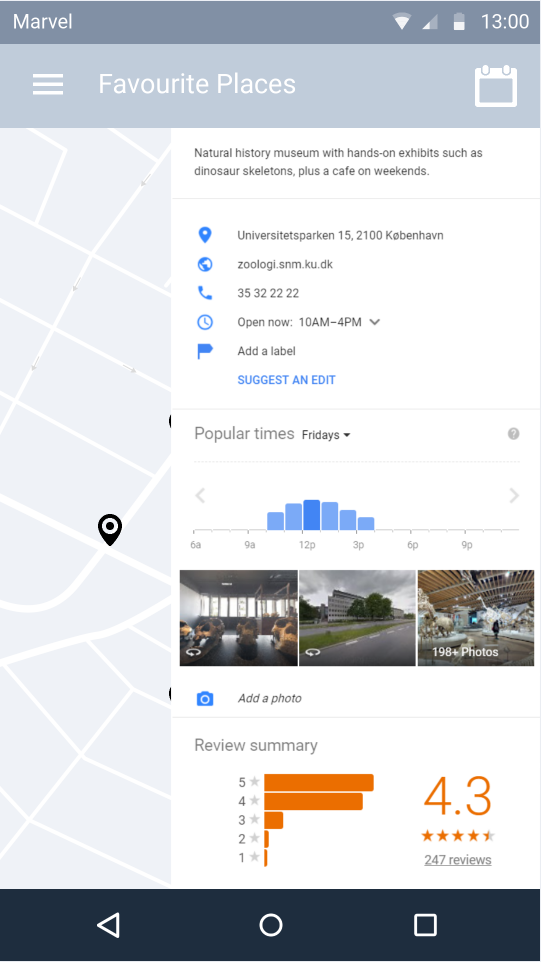
\includegraphics[height=8cm,keepaspectratio]{pics/app_design/fav_places.PNG}
                \caption{Sketch of Favourite Places}
            \end{figure}
    		
    		\subsection{Advice}
    		There is also an option to access individual advice, such as what different routes could you take to get to your desired destination faster, what would be the best time to visit a specific location of your choice, what other locations would you rather want to go to that are closer to your location, among many other things. Plus, you can turn on a warning that reminds you to go outside when the app notices that you are spending too much time indoors.
    		
    	%----------------------------------------------------------------------------------------
		%   SOFTWARE ARCHITECTURE
		%----------------------------------------------------------------------------------------
    		
    	\newpage
    	\section{Software Architecture}

		%----------------------------------------------------------------------------------------
		%   IMPLEMENTATION
		%----------------------------------------------------------------------------------------
		    
		\newpage
		\section{Implementation} \label{sec:Implementation}
		
		    \subsection{Introduction}
		    We used \textit{Android Studio} as the development IDE and \textit{Java} as the programming language. Furthermore, we used \textit{Git} for version control. The source code of this application can be viewed on \textit{GitHub} \cite{repo}.
		    
		    This project relies heavily on Google Application programming interfaces (API) \cite{GoogleDevProducts} and built-in Android libraries. A library we relied heavily on was the Java Client for Google Maps Services \cite{JavaGoogleAPI}. Most of the APIs Google offers are intended to be used as JavaScript services, however, the aforementioned library adds a Java client which provides access to the API endpoints.
            Due to the absence of funds when creating this project we were forced to use the free versions of Google's APIs which have usage quotas. The Geocoding API, for example, is limited to
            \cite{GeoCodingAPILimits}:
            
            \begin{itemize}
                \item 2,500 free requests per day, calculated as the sum of client-side and server-side queries
                \item 50 requests per second, calculated as the sum of client-side and server-side queries
            \end{itemize}
            
            Considering that it's expected four users to have in excess of 100000 coordinates recorded (the amount depends on the individual user's settings), these limits make the app very slow and limits its capabilities. Nevertheless, the APIs provided a quick and easy way to implement the features we wanted to include in a usable manner.
            
            \subsection{Introduction slides}
            
            \begin{figure}[ht]
    		    \center
                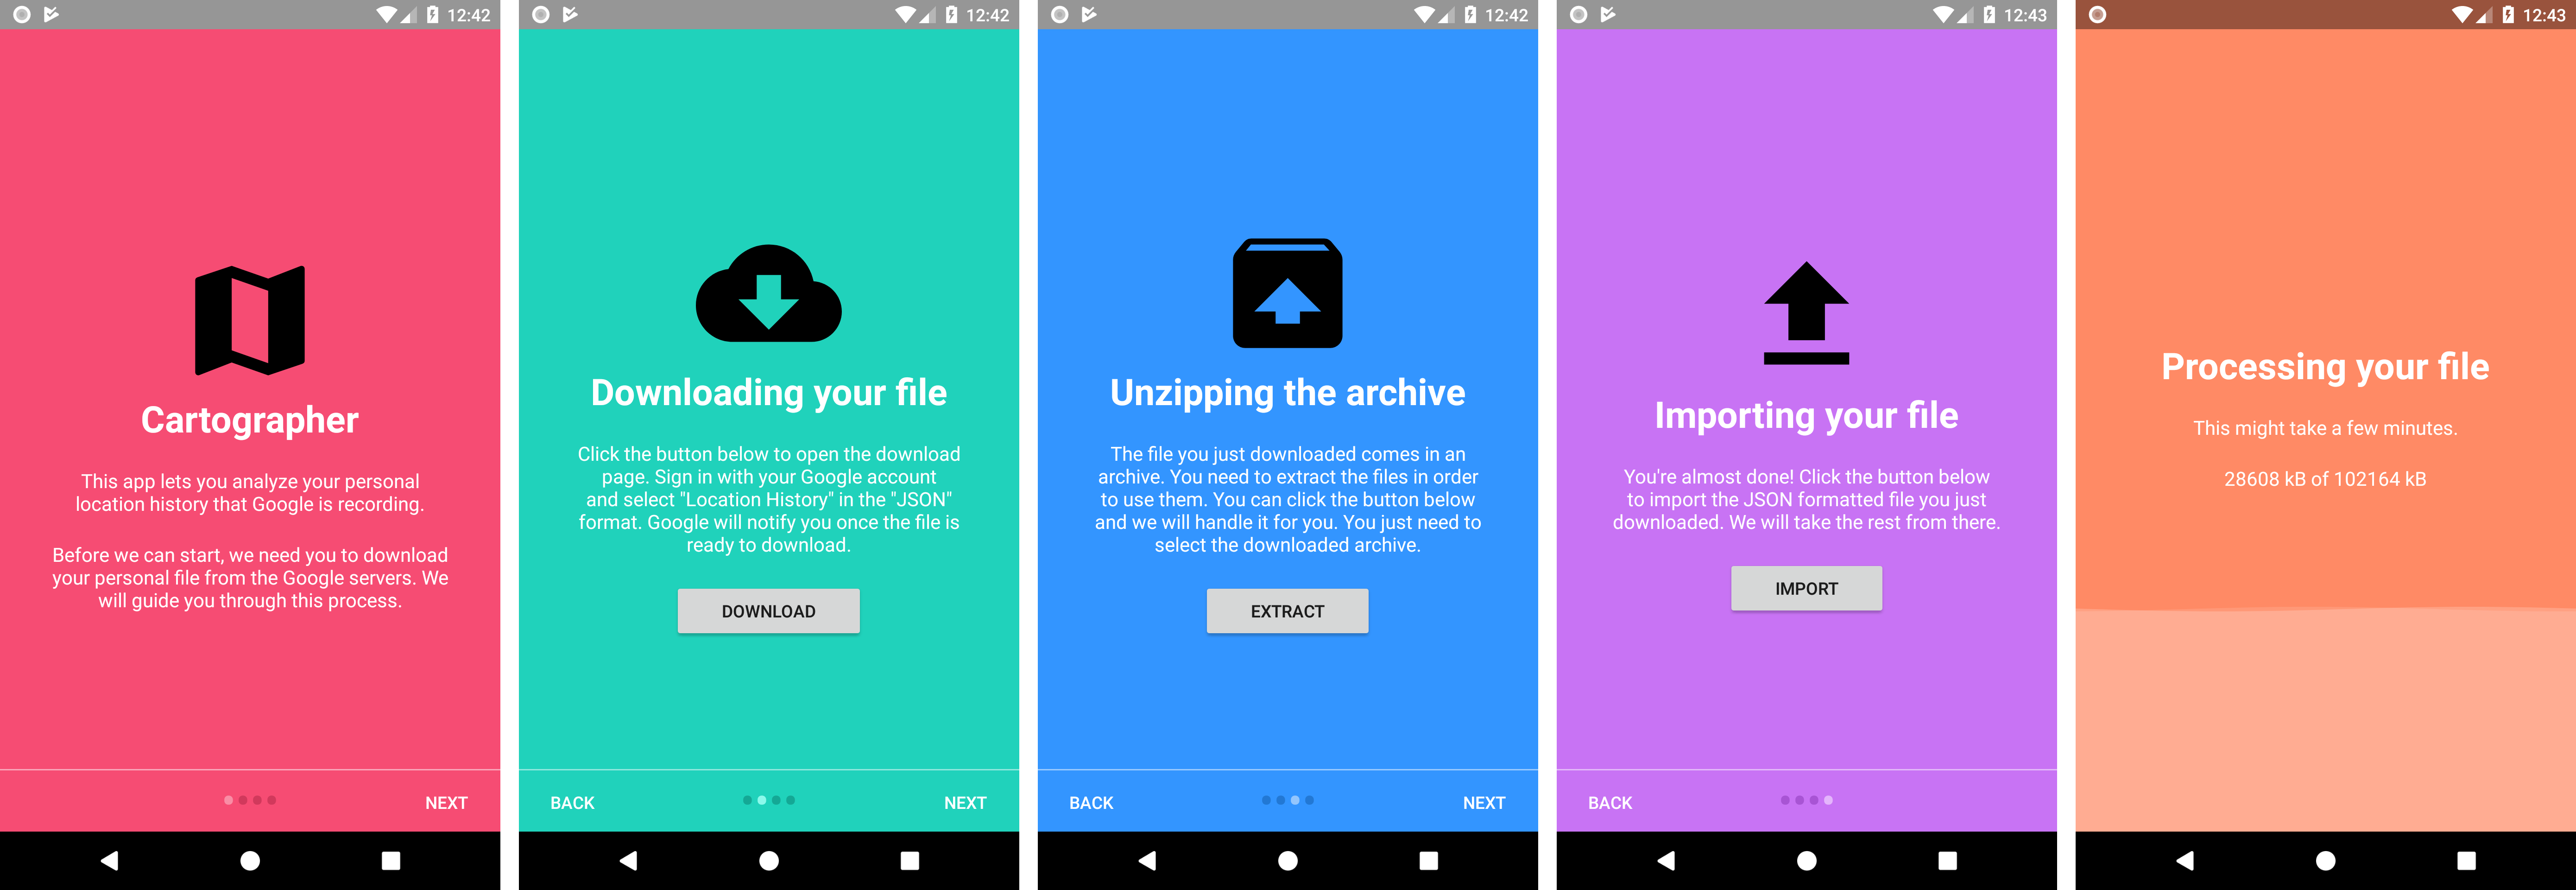
\includegraphics[width=1\textwidth]{pics/app_design/intro_slides_comp}
                \caption{Introduction slides}
                \label{fig:introduction_slides}
            \end{figure}
            
            There are many Android libraries for introduction slides, such as \textit{AppIntro} \cite{AppIntro} or \textit{Material Intro Screen} \cite{MaterialIntroScreen}. However, while testing out those two libraries, among others, we quickly noticed some problems regarding bugs and usability, as well as the fact that some libraries are outdated and should therefore not be used. 
            
            An alternative was quickly found in a tutorial on \textit{Android Hive} \cite{IntroSlidesTutorial} that shows how to implement your own, custom introduction slides. This helped us a lot with setting up the slides. However, we changed several parts of the source code from the tutorial. For example, we didn't want to have a \textit{Skip} button, because the user is required to upload a file before he or she can proceed. Because of this, we reworked this button to be a \textit{Back} button. All final slides can be seen in Figure \ref{fig:introduction_slides}.
            
            The custom introduction slides also caused some issues with the \texttt{ViewPager} widget, because the UI elements on some slides were visible, but not accessible. This was caused by the \texttt{ViewPager} not caching the next slide when navigating with the buttons instead of swiping. This took a long time to fix and we finally discovered that we can just preload every slide into the memory, instead of dynamically loading it on demand. This fixed our issue.
            
            As for the functionality of the slides, the \textit{Download} button opens the default browser and navigates to the Google Takeout page, which is the central repository where users can download their Google data.
            
            The \textit{Extract} button on the third slide opens a file browser and asks the user to select a \texttt{.zip} file, which will then be extracted to the same directory. For this, we used the Java library \textit{Zip4j} \cite{zip4j}.
            
            Finally, the \textit{Import} button on the last slide opens yet another file browser to select the \texttt{.json} file, which will then be processed by the app. Because the size of this file is usually of significant size ($\sim$100 MB for one year of data), a separate loading screen is shown while the file is being processed in the background. The loading animation in the background is a wave that is progressively filling up the screen while progressing. This widget is coming from the \textit{Wave View} library \cite{WaveView}.
            
            \subsection{File processing}
            
            Processing the JSON file was certainly one of the biggest programming tasks in the project. The file usually contains millions of lines of text and can be several hundreds of megabytes large. We had to find a way to parse this file fast without annoying the user if the process is too slow.
            
            There are many JSON libraries for Java, such as \textit{Jackson} \cite{Jackson},  \textit{GSON} \cite{Gson} and the native Java API \cite{JavaJsonNative}. We decided to use \textit{Gson} because we found it to be the easiest to use. Furthermore, it is developed by Google, which means that they most likely use it in the Android OS itself. Because of this, we are comfortable with using their library instead of others.
            
            A big problem with parsing such a big file is the memory. It is not possible to simply use the built-in functions of the library to read the whole file into the memory and receive some kind of output. This is highly inefficient and crashes the app if the file is too large. Because of this, we are using the \texttt{Json Reader} of the Gson library, which lets us read a JSON file token by token and decide ourselves, what to do with the values.
            
            This process is running in an asynchronous task so that the UI is not blocked and the loading screen can be updated. Another issue here was that we needed to calculate a percentage value of the progress in order to show it on the loading screen. The normal \texttt{Input Stream} in Java does not implement such a functionality, but we found a solution online \cite{ProgressInputStream}. This solution simply extended the normal \texttt{Input Stream} in Java and added a method to estimate the progress, by counting the processed bytes and dividing it by the full file size.
            
            \subsection{Database}
            
            The application stores the data from the user's JSON file in a database to have it available fast. Parsing the JSON file over and over again when the user requests to see the heatmap, for example, is highly inefficient.
            
            We chose SQLite as our database for several reasons. First of all, the database needs to be offline in order to comply with the entire project. It would be hypocritical to promote privacy on one hand, but then go ahead and store all the user's highly sensitive data online. There are plenty of offline databases available for Java/Android, but we only needed a simple way of storing the massive amount of data and be able to query it quickly again. We would have liked to use \textit{Realm} \cite{Realm}, but it is not available for free. The advantages of \textit{Realm} are that you can work with native objects instead of reading and writing single values from and to columns (as in SQL), as well as being able to easily encrypt the database with AES-256 encryption \cite{RealmFeatures}, which would be a big benefit to us, since we want to store the sensitive data as secure as possible. However, because it is not free, we stuck to SQLite due to its ease of use and high popularity, which means that there is plenty of documentation and support online.
            
            The database consists of several tables. The biggest and most important table is the entire data from the user's JSON file. This data is identical to the file's content, but available much faster because it is stored in a database and not the file. There are also smaller tables for features such as the favourite places. This table is being used to store the processed information from the main table so that not all data has to be analysed over and over again when using a feature.
            
            \subsection{Favourite places}
            
            \begin{figure}[ht]
                \center
                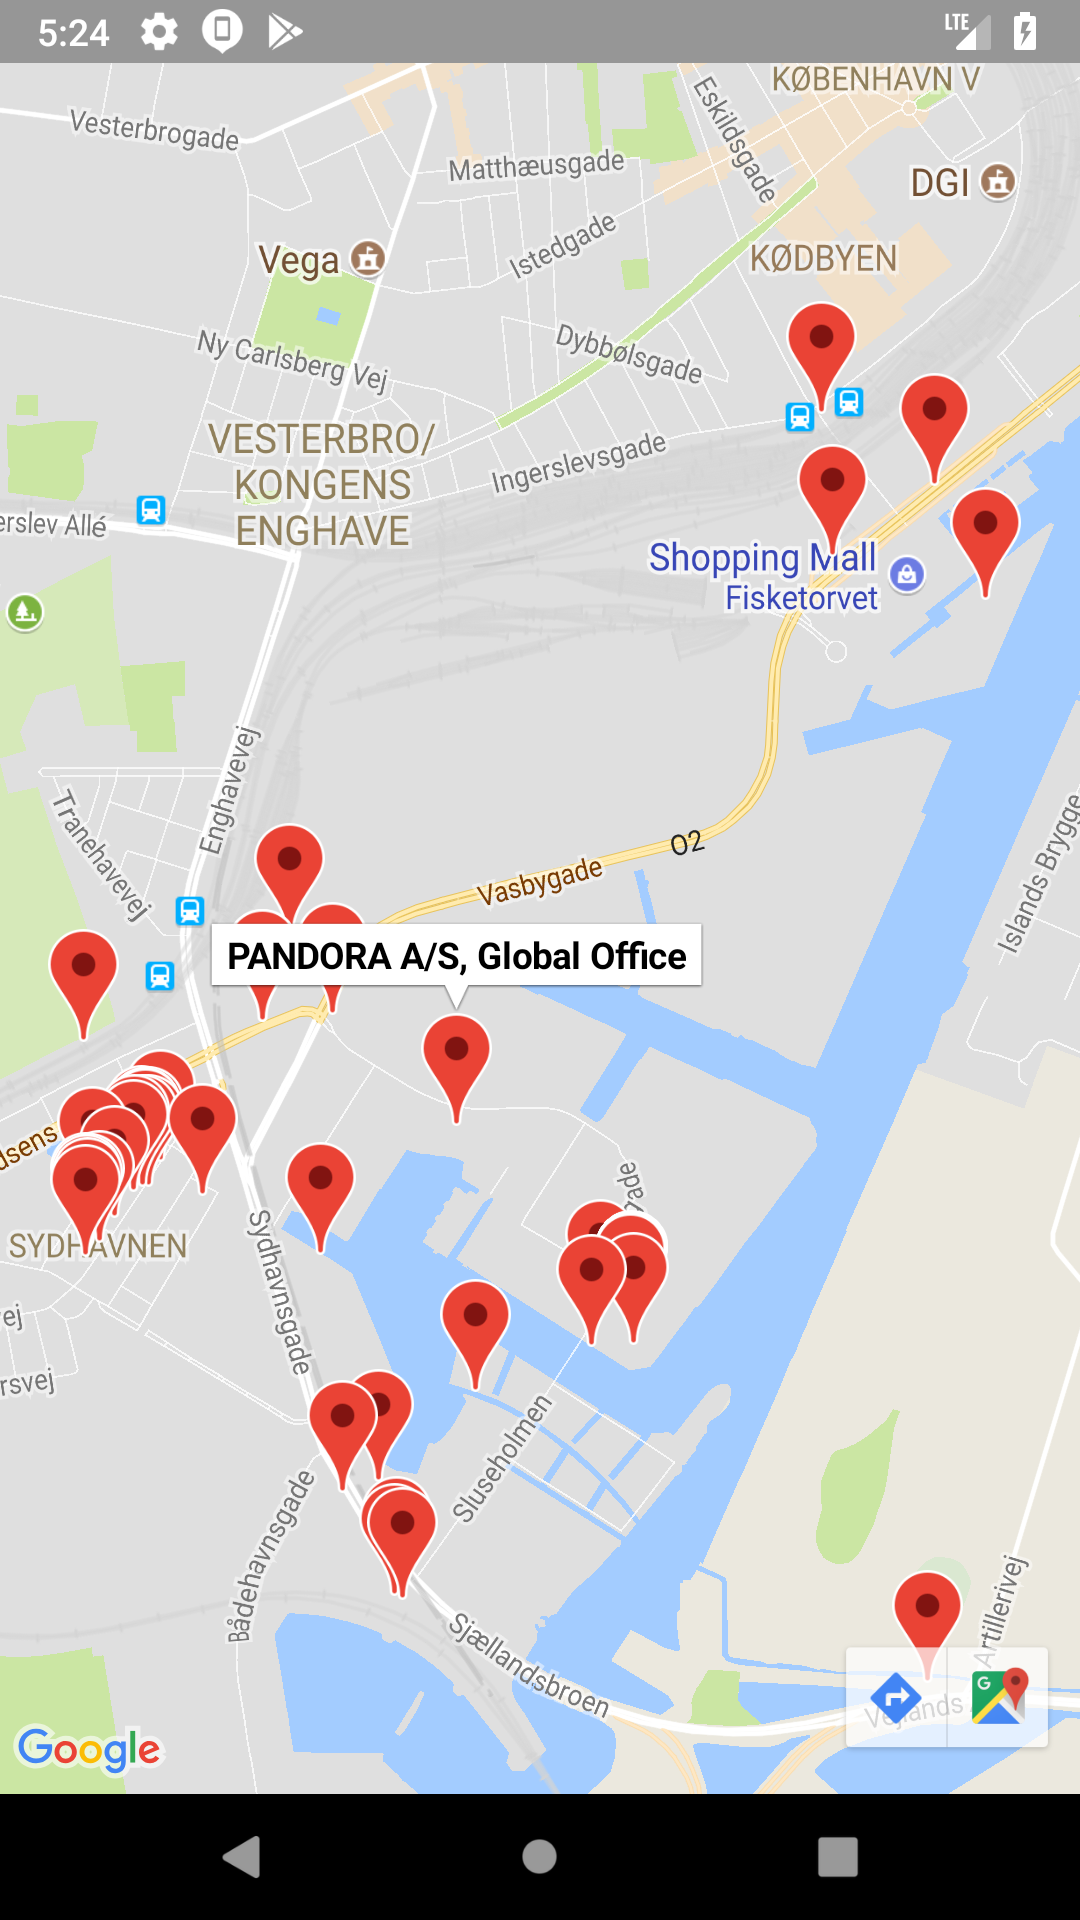
\includegraphics[height=8cm,keepaspectratio]{pics/fav-places-screenshot.png}
                \caption{Screenshot of Favourite Places}
            \end{figure}
            To generate the list of favourite places we had to go through all the data points a user has, check if some of them are duplicated and how many times. The data provided by the user though contains only the coordinates where they have been. To find out if they were actually in some kind of establishment (restaurant, supermarket, shopping mall, etc) we need to find out what places are nearby the user. 
            
            We accomplished this by using Google's Radar Search API \cite{GoogleRadarSearch}. It works by passing it a coordinate to the API and it returns a list of businesses that are near those coordinates. The most relevant result is stored in a table for the favourite places.
            
            The table is queried when rendering the favourite places view and the results are rendered as markers on a map. When a marker has been clicked, the name of the business located there.
		    
		    \subsection{Conclusion}
		
		%----------------------------------------------------------------------------------------
		%   USER RESEARCH
		%----------------------------------------------------------------------------------------
		
		\newpage
		\section{User Research} \label{sec:UserResearch}
		
		The online survey, which was described in the Methodology, gained an intermediate amount of traction, with about 50 answers, three weeks after publishing. There are no statistics of where participants come from, what their background is or what their age is. However, we can make an educated guess that around half the answers are from AAU students, and the other half from unknown persons that participated through one of the websites described in the Methodology. We can guess this, because there was a delay of a few days between posting the survey in the AAU project help Facebook group and submitting it to third party online survey services.
		
		\subsection{Android and Google Maps}
		
		The first step of the survey is to filter out irrelevant participants. Since this project is all about creating an Android application, we are mainly looking for Android users. However, other smartphone users are still relevant, if they use the Google Maps mobile app. Despite the Android market share of 75\% in 2017 \cite{SmartphoneOSMarketShare}, most participants were no Android users. In fact, only 22 out of 47 participants (46,8\%). This is most likely due to the higher market share of iOS in Denmark \cite{SmartphoneOSMarketShareDenmark} and the fact that most of our participants reside in Denmark.
		
		Out of the 25 non-Android users, only 4 participants answered that they don't have the Google Maps mobile application installed on their phone. In total, only 4 out of 47 (around 8\%) were irrelevant for the survey.
		
		\subsection{Knowledge of location related data collection}
	    
	    \begin{wrapfigure}{r}{0.5\textwidth}
          \begin{center}
            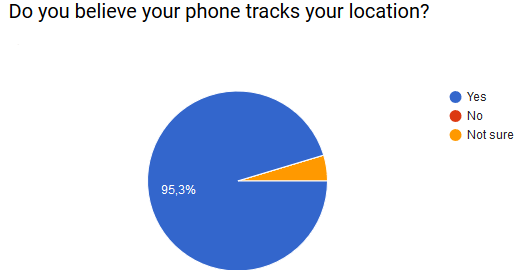
\includegraphics[width=0.5\textwidth]{survey/survey1}
          \end{center}
          \caption{Survey question: location tracking}
          \label{fig:survey_location_tracking}
        \end{wrapfigure}
	    
	    This section of the survey focuses on the knowledge and awareness that the participant has about location tracking. The first question (see figure \ref{fig:survey_location_tracking}) asks whether the participant believes that his or her phone is tracking the phone's location. This was overwhelmingly answered with "Yes". Nobody has answered "No", and only two participants weren't sure. This goes to show that everyone is very aware of this kind of behaviour nowadays, which is most likely caused by the many privacy scandals of the past years, not only related to location tracking.
        
        Going more into detail, fewer people know actual details on this subject. To the question \textit{"Do you believe that this location data is accessible to you as a user?"}, only 75\% think that the data is indeed accessible (speaking of Google Maps). Furthermore, only 37\% have ever seen the location history that Google has recorded of them. This 37\% mostly viewed their location history on the Google Maps website or mobile application (coming from a text answer field).
		
		\subsection{Cartographer}
		
		The last section now focuses on the application that we built within this project. We wanted to know if people are at all willing to use such an application and if they do, what features they would like the application to have.
		
		Only every third participant was not interested in such an application, meaning that 67\% (29 out of 43 participants) were interested. Those people that were not interested received one more final question which was aimed to ask for the reason. Half of those participants answered that they had privacy concerns and the other half simply did not care enough about the subject.
		
		Going further, we asked how comfortable the participant is with sharing their full location history with the application and therefore an unknown third-party provider. The results on this were very mixed, with a few people completely mistrusting the application, and a lot of people somewhere in the middle ranks (see figure \ref{fig:survey_location_access}).
		
		\begin{figure}[ht]
            \center
            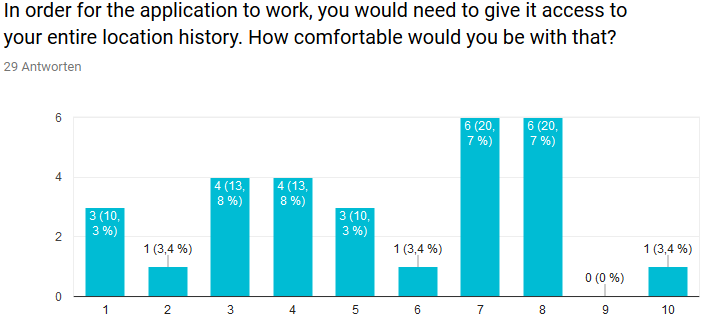
\includegraphics[width=1\textwidth]{survey/survey2}
            \caption{Survey: Access to the location history}
            \label{fig:survey_location_access}
        \end{figure}
        
        When asking for the desired functionalities of the application, 97\% (everyone except one) of participants want to see their most frequent routes. 62\% want to have an overview of their most visited places, and 51\% want to have heat maps of their overall location history. Furthermore, 86\% want to get advice on how to improve their routes, and 69\% would like to get additional information about their most frequently visited places.
		
		\subsection{Conclusion}
		
		The answers to the questionnaire paint a clear picture that most people are aware of data collection practices by major companies such as Google. However, many people don't know much more than the fact that they're being "watched". The survey shows that many participants haven't even seen the data that is being collected on them, or is aware that they are able to see it.
		
		This lack of awareness helps greatly with the demand of our application, because many are curious, what data is actually being collected on them. However, the survey also shows that many participants have concerns about the application's privacy practices and are unsure about it's trustworthiness. Because of this, it is important for us to be transparent and honest about our privacy policy and data handling.
		
		The full survey with all questions and answers can be seen in Appendix \ref{FullSurvey}.
		
		%----------------------------------------------------------------------------------------
		%	FUTURE
		%----------------------------------------------------------------------------------------
		
		\newpage
		\section{Future} \label{sec:Future}
		
		Explain the future of this project and how the technology might evolve
		
		%----------------------------------------------------------------------------------------
		%	CONCLUSION
		%----------------------------------------------------------------------------------------
		
		\newpage
		\section{Conclusion} \label{sec:Conclusion}
		
		%----------------------------------------------------------------------------------------
		%	BIBLIOGRAPHY
		%----------------------------------------------------------------------------------------
		
		\newpage
		\printbibliography[heading=bibintoc,title={References}]
		
		%----------------------------------------------------------------------------------------
		%	APPENDIX
		%----------------------------------------------------------------------------------------
		
		\newpage
		\appendix
		
		\section{Appendix}
		
		\subsection{Survey} \label{FullSurvey}
		
		The following questions and answers show the full survey in text form.
		
		\begin{enumerate}
		    \item Are you an Android user?
		    \begin{itemize}
		        \item Yes (25 answers, 53,2\%)
		        \item No (22 answers, 46,8\%)
		    \end{itemize}
		    
		    \item Do you have the Google Maps application installed on your phone?
		    \\\textit{Only displayed if answer was "No" in previous question.}
		    \\\textit{Answering "No" ends the survey.}
		    \begin{itemize}
		        \item Yes (21 answers, 84\%)
		        \item No (4 answers, 16\%)
		    \end{itemize}
		    
		    \item Do you believe your phone tracks your location?
		    \begin{itemize}
		        \item Yes (41 answers, 95,3\%)
		        \item No (0 answers, 0\%)
		        \item Not sure (2 answers, 4,7\%)
		    \end{itemize}
		    
		    \item Do you believe that this location data is accessible to you as a user?
		    \begin{itemize}
		        \item Yes (32 answers, 74,4\%)
		        \item No (11 answers, 25,6\%)
		    \end{itemize}
		    
		    \item Have you ever seen the location history that Google has recorded on you?
		    \begin{itemize}
		        \item Yes (16 answers, 37,2\%)
		        \item No (27 answers, 62,8\%)
		    \end{itemize}
		    
		    \item If yes, how did you gain access and in what format did you view it?
		    \begin{itemize}
		        \item Google Maps web \& mobile app
		        \item Third party services
		        \item Viewed it on my laptop, google maps
		        \item Google send a message
		        \item Google Maps mobile + desktop 
		        \item Google maps shows me where i've been and when, but when i turn it off, i use a GPS mocker, and just place it at home. google maps thinks i'm home, snapchat thinks i'm home so privacy (even tho it's kinda a walk around)
		        \item Google Maps
		        \item computer
		        \item Google Maps, Google+
		        \item Google Maps mobile app
		        \item Laptop
		        \item Google Maps Timeline (mobile, desktop), Google Fit (mobile), Google Search and Search History (mobile), Google Settings (desktop when logged in) + several mobile apps that implement a location feature
		        \item I used Google Timeline and Takeout
		    \end{itemize}
		    
		    \item Would you be willing to use an application that can present you an in-depth analysis of your location history?
		    \begin{itemize}
		        \item Yes (29 answers, 67,4\%)
		        \item No (14 answers, 32,6\%)
		    \end{itemize}
		    
		    \item Why not?
		    \\\textit{This question is only displayed if the previous answer was "No". The survey ends after this question.}
		    \begin{itemize}
		        \item Privacy concerns (7 answers, 50\%)
		        \item I don't care (6 answers, 42,9\%)
		        \item I don't care since it wont affect Google tracking my location either way. If it blocked the data gathering from google then yes. (1 answer, 7,1\%)
		    \end{itemize}
		    
		    \item In order for the application to work, you would need to give it access to your entire location history. How comfortable would you be with that?
		    \\\textit{The answers are on a scale from 1 to 10, with 10 being the most comfortable.}
		    \begin{itemize}
		        \item 10 (1 answer, 3,4\%)
		        \item 9 (0 answers, 0\%)
		        \item 8 (6 answers, 20,7\%)
		        \item 7 (6 answers, 20,7\%)
		        \item 6 (1 answer, 3,4\%)
		        \item 5 (3 answers, 10,3\%)
		        \item 4 (4 answers, 13,8\%)
		        \item 3 (4 answers, 13,8\%)
		        \item 2 (1 answer, 3,4\%)
		        \item 1 (3 answers, 10,3\%)
		    \end{itemize}

		    \item What functionality would you like the app to have?
		    \\\textit{This is a multiple choice question. The percentage shows how many participants want a certain feature.}
		    \begin{itemize}
		        \item Heat maps (15 answers, 51,7\%)
		        \item Most visited places (18 answers, 62,1\%)
		        \item Most frequent routes (28 answers, 96,6\%)
		    \end{itemize}
		    
		    \item Would you like to get advice on how to improve your commute?
		    \begin{itemize}
		        \item Yes (25 answers, 86,2\%)
		        \item No (4 answers, 13,8\%)
		    \end{itemize}
		    
		    \item Would you like to get additional information about your most frequently visited places?
		    \begin{itemize}
		        \item Yes (20 answers, 69\%)
		        \item No (9 answers, 31\%)
		    \end{itemize}
		\end{enumerate}
		
		%------------------------------------------------
		
\end{document}